\documentclass[twoside]{article}
\usepackage{aistats2022}
% If your paper is accepted, change the options for the package
% aistats2022 as follows:
%\usepackage[accepted]{aistats2022}

% If you set papersize explicitly, activate the following three lines:
%\special{papersize = 8.5in, 11in}
%\setlength{\pdfpageheight}{11in}
%\setlength{\pdfpagewidth}{8.5in}

% If you use natbib package, activate the following three lines:
\usepackage[round]{natbib}
\renewcommand{\bibname}{References}
\renewcommand{\bibsection}{\subsubsection*{\bibname}}

\usepackage[utf8]{inputenc} % allow utf-8 input
\usepackage[T1]{fontenc}    % use 8-bit T1 fonts
\usepackage{hyperref}       % hyperlinks
\usepackage{url}            % simple URL typesetting
\usepackage{booktabs}       % professional-quality tables
\usepackage{microtype}      % microtypography
\usepackage{graphicx}
\graphicspath{{../figs/}{../}}
%\usepackage{subfigure}
\usepackage{subcaption}
\usepackage{hyperref}       % hyperlinks
\usepackage[dvipsnames]{xcolor}

\hypersetup{ % SLJ: my standard paper setup...
	pdftitle={MAP convergence},
	pdfkeywords={},
	pdfborder=0 0 0,
	pdfpagemode=UseNone,
	colorlinks=true,
	linkcolor=blue, %mydarkblue,
	citecolor=blue, %mydarkblue,
	filecolor=blue, %mydarkblue,
	urlcolor=blue, %mydarkblue,
	pdfview=FitH,
	pdfauthor={Anonymous},
}


\newcommand{\RLP}[1]{\textcolor{red}{RLP:#1}}
\newcommand{\fdk}[1]{\textcolor{Periwinkle}{fdk:#1}}
\newcommand{\TODO}[1]{\textcolor{cyan}{TODO #1}}

% my packages
\usepackage{../math_commands}
% some custom math commands
\newtheorem{proposition}{Proposition}
\newcommand*{\expect}[2][]{\ensuremath{\mathbb{E}_{#1} \left[ #2 \right] }} % expectation operator
\newcommand{\logpart}{A}
\newcommand{\conj}{\logpart^*}
\newcommand{\bregman}{\cB_\logpart}
\newcommand{\bregmanconj}{\cB_{\logpart^*}}
\newcommand{\natp}{\theta}
\newcommand{\meanp}{\mu}
\newcommand{\decrement}{D}
\newcommand{\linear}{\ell} % linearization of a function
\newcommand{\lr}{\gamma} % learning rate, or step-size
\newcommand{\lin}[1]{\left\langle#1\right\rangle}

\newcommand{\MAPm}{\hat \mu_n}
\newcommand{\MAPt}{\hat \natp_n}


\begin{document}

% If your paper is accepted and the title of your paper is very long,
% the style will print as headings an error message. Use the following
% command to supply a shorter title of your paper so that it can be
% used as headings.
%
%\runningtitle{I use this title instead because the last one was very long}

% If your paper is accepted and the number of authors is large, the
% style will print as headings an error message. Use the following
% command to supply a shorter version of the authors names so that
% they can be used as headings (for example, use only the surnames)
%
%\runningauthor{Surname 1, Surname 2, Surname 3, ...., Surname n}

\twocolumn[

\aistatstitle{Looking for Convergence Rates\\ for the MAP of the Exponential Family}


\aistatsauthor{R\'emi Le Priol \And Frederik Kunstner \And  Damien Scieur \And Simon Lacoste-Julien }

\aistatsaddress{ Mila \And  UBC \And SAIT SAIL \And Mila} 
]

\begin{abstract}
We consider the problem of upper bounding the expected sub-optimality of the maximum likelihood estimate (MLE), or a conjugate maximum a posteriori (MAP) for the exponential family. 
Surprisingly, we found no solution to this problem in the literature -- e.g. after seeing 5 samples, we do not know how many bits away (in expectation) our model is from the true distribution.
After displaying some properties and special cases of this problem, 
we show it is an application of several optimization algorithms.
Yet it falls out of scope for current analysis, thus highlighting areas for progress.
\end{abstract}

\section{Introduction and Background}

\fdk{Consider the optimization of 
\begin{equation}
	f(\theta) = \expect[x \sim p(x)]{\frac{1}{2}\norm{\theta}^2 - \lin{x, \theta}},
\end{equation}
given samples from $x$. We know how to do that one, 
and the worst-case scenario happens when $p(x)$ is a Gaussian.
Now how about the slightly more general case where
\begin{equation}
	f(\theta) = \expect[x \sim p(x)]{A(\theta) - \lin{x, \theta}}
\end{equation}
and we have full knowledge of $A$, a strictly convex twice differentiable function. 
How hard can that be?
Turns out, if $p$ is the maximum entropy distribution with 
$\expect[x \sim p(x)]{x} = \mu$, 
then it's a bit hard.}

Call both to stats and optimization crowds by introducing the parallel quite early.


\RLP{Goal = disseminate related work to make it look nice.}
Exponential Families are an elegant and lean way to model a wide variety of data : binary, categorical, natural numbers, positive float, long or short tailed... 
They are literally the linear model of probabilities.
The exponential family for data $X$ with natural parameter $\natp$  is entirely specified by the support set of the data   $\cX$ and a sufficient statistic $T: \cX \rightarrow \real^d$
\begin{equation}
	 p(X|\natp) = \exp( \natp^\top T(X) - \logpart(\natp)) \; ,
\end{equation}
where $\logpart$ is the log-partition function -- i.e. the normalization factor
\begin{align}
    \logpart(\natp) = \log \int e^{\natp^\top T(x)} dx 
\end{align}
where the integral stands for a sum if $x$ has discrete support. \RLP{Use base measure instead.}
For instance, this simple model encompasses both categorical distributions $\cX = \{1, \dots, k\}$ with $T(X)$ being the one-hot encoding, and multivariate normal distributions $\cX=\real, T(X)=(X, X^2)$. 

\paragraph{Duality}
The logpartition function $\logpart$ verifies the two following identities
\begin{align}
    \nabla\logpart(\natp) &=  \expect[p(X|\natp)]{T(X)} =: \meanp \\
    \nabla^2 \logpart(\natp) &= \Cov_\natp[T(X)] > 0
\end{align}
where $\meanp$ is called the mean parameter.
If the sufficient statistic $T$ is minimal, then the log-partition function $\logpart$ is strictly convex and its gradient $\nabla \logpart$ is a bijection between natural parameters $\natp$ and mean parameters $\mu$.
We will write indifferently $\mu$ or  $\natp$ depending on the context, being aware that both represent the same distribution.
The second identity entails that $\logpart$ is strictly-convex. 
At this point it is useful to introduce the \href{https://en.wikipedia.org/wiki/Convex_conjugate}{convex conjugate} (aka Fenchel-Legendre transform) of the logpartition function
\begin{align}
	\conj(\mu) = \langle \mu, \natp \rangle - \logpart(\natp) \; .
\end{align}
which matches the common notion of \textit{entropy} in information theory.
If $\logpart$ is strictly convex, then its gradient is strictly monotone, so it is a bijection, and its inverse is the gradient of its dual $\nabla\conj \circ \nabla\logpart(\natp) = \natp$ (cf Fig.~\ref{fig:duality}).
For a full review of exponential families and their duality, see \citet[Chapter 3]{wainwright2008graphical}.
\begin{figure}[ht]
	\centering
	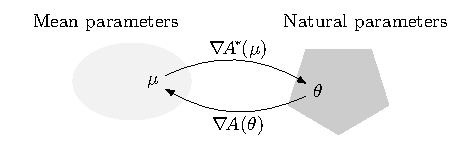
\includegraphics{duality}
	\caption{The gradient of the log-partition function and its dual, $(\nabla \logpart, \nabla \conj)$, form a bijection between the natural and mean parameters $\natp, \meanp$. Figure reproduced from \citet{kunstner2020homeomorphic}.
		\RLP{Show the true gaussian bijection instead?}
	}
	\label{fig:duality}
\end{figure}

\paragraph{Conjugate Prior}
One conjugate prior for $p(X|\natp)$ is
\begin{align}
    p(\natp) &\propto \exp( - n_0 \bregman(\natp ; \natp_0) )
\end{align}
where $n_0$ and $\natp_0$ are (hyper)parameters of the prior, and $\bregman(\natp ; \natp_0)$ is the Bregman divergence induced by $\logpart$ between $\natp$ and $\natp_0$
\begin{align}
    \bregman (\natp ; \natp_0)
    & = \logpart(\natp) - \logpart(\natp_0) 
    - \langle \nabla \logpart(\natp_0)  , \natp - \natp_0 \rangle
\end{align}
with $\nabla \logpart(\natp_0) = \expect[\natp_0]{T(X)} =: \meanp_0$ the mean parameter associated to $\natp_0$. 
Intuitively, $n_0$ is a number of fictive points observed from a distribution with parameter $\natp_0$.
We can re-write this prior as 
\begin{align}
    p(\natp) \propto 
    \exp( -n_0 \logpart (\natp) 
    + \langle n_0 \mu_0, \natp \rangle ) \; ,
\end{align}
which is the formula for the exponential family with sufficient statistics $(\natp ,\logpart(\natp))$ and with natural parameter $(n_0 \mu_0, -n_0)$.
The posterior given $\cD=(X_1,\dots, X_n)$ is then part of the same family, with natural parameters $(n_0 \mu_0 + \sum_i T(X_i) , -(n_0 + n))$.

\paragraph{Maximum A Posteriori (MAP).}
The negative log-likelihood of the prior is
\begin{align*}
    -\log p(\natp) = n_0 (\logpart(\natp)  - \natp^\top \meanp_0 ) + \cst
\end{align*}
Thus the joint log-likelihood of $\cD =(X_1,\dots,X_n,\natp)$ is
\begin{multline}
    -\log p(\cD|\natp)p(\natp) 
    = (n_0+n) \logpart (\natp) \\
    - \theta^\top \left(n_0 \meanp_0 + \sum_{i=1}^n T(X_i) \right) + \cst \; .
\end{multline}
Minimizing this expression over $\natp$ yields the Maximum A Posteriori estimate
\begin{align}
    \hat \natp = \argmin_\natp -\log p(\cD|\natp) + n_0 \bregman(\natp ; \natp_0)
\end{align}
such that the MAP is
\begin{align}
    \nabla \logpart(\hat \natp_\text{MAP}) = \hat \meanp_\text{MAP}
    = \frac{n_0 \meanp_0 + \sum_{i=1}^n T(X_i) }{n_0+n} \; .
\end{align}
When $n_0=0$ -- eg we observed zero samples from the prior -- we recover the Maximum Likelihood Estimate (MLE)
\begin{align}
	\hat \mu_\text{MLE} = \frac{\sum_{i=1}^n T(X_i)}{n}
\end{align}
The MLE and MAP estimates are statistics of the dataset $\cD$. Given a random dataset, we wish to bound their deviation from the optimum $\natp^*$ or $\meanp^*$.


\section{Open Problem}

For a well-specified model, the suboptimality on the population log-likelihood is exactly the KL between our current model and the true distribution
\begin{multline}
    \expect[X\sim p(.|\natp^*)]{-\log p(X|\natp) + \log p(X|\natp^*) } \\
	= \KL( p(.|\natp^*) ; p(.|\natp)) \; .
\end{multline}
For the exponential family, the KL is equal to the Bregman divergence induced by the log-partition function, or alternatively by the entropy, being careful with the order of the arguments 
\begin{align}
\boxed{
	\KL( p(.|\natp^*) ; p(.|\natp))
    = \bregman (\natp ; \natp^*)
    = \bregmanconj ( \meanp^* ; \meanp)
}
\end{align}
Our question is: how does this quantity behave when $\natp$ is the maximum-likelihood or the MAP estimate ? Can we get upper-bounds on the following quantities
\begin{align}
	\label{eq:bregmanMLE}
	\expect[\cD]{\bregmanconj \left (\E [T(X)] ;  \inv{n}  \smallsum_i T(X_i) \right )} \\
	\label{eq:bregmanMAP}
	\expect[\cD]{\bregmanconj \left (\E [T(X)] ; \frac{n_0 \mu_0 + \smallsum_i T(X_i)}{n_0+n} \right )} 
\end{align}
where the outer expectation is on the dataset $\cD = \{X_1, \dots, X_n \}$ sampled i.i.d as $X_i\sim \natp^*$?


\paragraph{Remark.}
This could be seen as a concentration inequality, expressed with a Bregman divergence instead of a norm.
A key difference though, is that the random variable $T(X)$ is connected to the metric $\logpart$. 
Indeed expressions~\eqref{eq:bregmanMLE} or~\eqref{eq:bregmanMAP} can be infinite for another choice of random variable. 
For instance, if we plug in $\conj(\mu)= -\log(\mu)$, which defines a divergence on positive numbers, and $T(X) \sim \cN(0,1)$ which can be negative.

\paragraph{Remark 2.}
The expectation of the MLE may be infinite, for instance with $\cN(0,\sigma^2)$ and $n\leq 2$. Instead of taking the expectation,  we might want to bound this quantity in high probability, without resorting to Markov inequality, but that is a difficult endeavor.

\section{Examples}
\subsection{Gaussian Mean}

\subsection{Gaussian Variance}
The trailing example of this paper is a centered gaussian with unknown variance $\cN(0,\sigma^2)$.
The density of a centered normal variable is
\begin{align}
	p(x) = \inv{\sqrt{2\pi \sigma^2}} e^{-\frac{x^2}{2 \sigma^2}} \; .
\end{align}
Defining $T(X)=X^2$ as the sufficient statistic, we get natural parameter $\natp = -\inv{2 \sigma^2} <0$, and mean parameter $\mu=\E[T(X)] = \sigma^2 >0$. 
Mean and natural parameters are roughly inverse of each other
\begin{align}
	\natp = -\inv{2 \mu}\; .
\end{align}
Now we can match the log-likelihood with the exponential family template to get the log-partition function.
\begin{align}
	\log p(x) = - \frac{x^2}{2 \sigma^2} - \half \log(2 \pi \sigma^2 ) 
	= x^2 \natp - \logpart(\natp) \\
	\implies \logpart (\natp) = - \half \log(-\natp)  + \half \log(\pi) 
\end{align}

We can use the formula $\conj(\mu) = \mu \natp - \logpart(\natp)$ to get the entropy
\begin{align}
	\conj(\mu) = \half\left( -\log(\mu) + \log\frac{\pi}{2} - 1 \right) \; .
\end{align}
We can also take gradient and derivative of $\logpart(\natp)$ to retrieve the mean and covariance of the sufficient statistic $X^2$
\begin{align}
	\nabla\logpart(\natp) &= \frac{-1}{2 \natp} = \sigma^2 = \mu = \E[X^2] \\
	\nabla^2\logpart(\natp) &= \frac{1}{2 \natp^2} = 2 \sigma^4 = 2 \mu^2 = \Var(X^2) 
\end{align}
which we confirm thank to wikipedia since $\E[X^4] = 3 \sigma^4$ and thus $\Var(X^2) = \E[X^4] - \E[X^2]^2 = 3 \sigma^4 - \sigma^4 = 2 \sigma^4$.


The logpartition function is $\logpart(\natp) = -\log(-\natp) /2 + \cst$, thus the conjugate prior is the exponential family with sufficient statistic $(\natp, \log(-\natp) )$, eg a negative \href{https://en.wikipedia.org/wiki/Gamma_distribution}{Gamma distribution}.
In particular,
\begin{align}
	p(\natp) 
	&\propto 
    \exp( -n_0 \logpart (\natp) 
    + \langle n_0 \mu_0, \natp \rangle ) \\
    &\propto \exp( \half[n_0] \log(-\natp) + n_0\mu_0 \natp ) \\
	&\propto (-\natp)^{1 + \half[n_0] -1 } e^{-n_0 \mu_0 (-\natp)} / Z
\end{align}
from which we infer the shape parameter $\alpha=1 + \half[n_0]$ and the rate parameter $\beta = n_0 \mu_0$, eg $\natp \sim \Gamma (1+\half[n_0] , n_0 \mu_0)$. After seeing $n$ samples, the posterior is $\Gamma\left(1+\half[n_0+n] , n_0 \mu_0 + \sum_i T(X_i) \right)$.

Both the entropy and the log-partition are roughly negative logarithm $z\mapsto - \log(z)$. Which yields the same shape of Bregman divergence, as visible below (all three lines are equal)
\begin{align}
	\KL( \sigma_*^2 ; \sigma_n^2 ) 
	&= \half \left ( \frac{\sigma_*^2}{ \sigma_n^2} - 1 - \log \frac{\sigma_*^2}{ \sigma_n^2} \right) \\
	\bregmanconj( \mu_*; \mu_n) 
	&= \half \left ( \frac{\mu_*}{ \mu_n} - 1 - \log  \frac{\mu_*}{ \mu_n} \right) \\
	\bregman( \natp_n; \natp_* ) 
	&=  \half \left ( \frac{ \natp_n}{\natp_*} - 1 - \log  \frac{ \natp_n}{\natp_*} \right) \; .
\end{align}

In other words, this divergence measures the discrepancy between the ratio $\frac{ \natp_n}{\natp_*} =  \frac{\mu_*}{ \mu_n}  $ and $1$ via the function $\phi$
\begin{align}
	\phi(z) := \half (z - 1 - \log(z)) \\
	\bregman( \natp_n; \natp_* )   = \phi(\frac{ \natp_n}{\natp_*}) =  \phi(\frac{\mu_*}{ \mu_n})
\end{align}
as illustrated in Figure~\ref{fig:phi}. We can get a non-transcendental upper bound thanks to the inequality
\begin{align}
	1 - \inv{z} \leq \log(z) 
	\label{eq:log_bound} 
	\implies \phi(z) \leq \half (z + \inv{z}) - 1 = \frac{(z-1)^2}{2 z} \; .
\end{align}


\begin{figure}[ht]
	\centering
	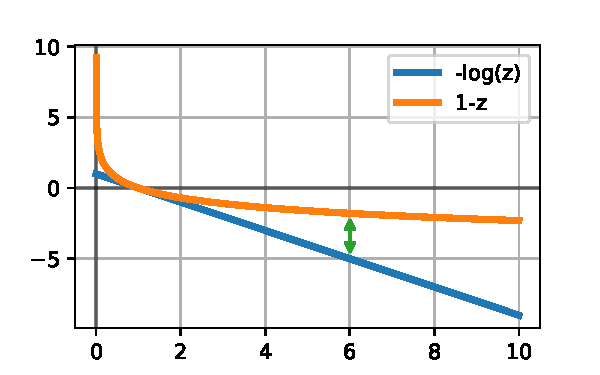
\includegraphics[width=.4\textwidth]{bregmandef.pdf}
	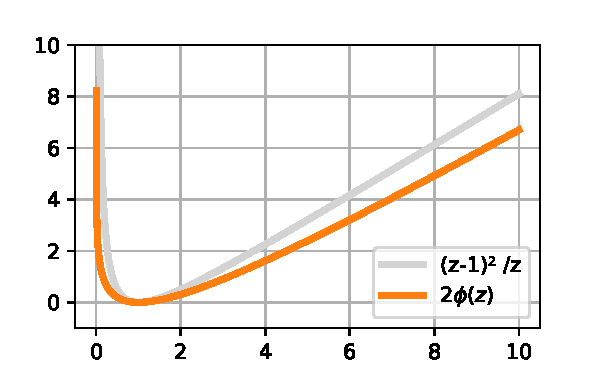
\includegraphics[width=.4\textwidth]{phi.pdf}
	\caption{$\phi(z)$ is the Bregman divergence induced by $-\log(z)$. It is a barrier near $0$. As a result, it is poorly approximated by quadratics.}
	\label{fig:phi}
\end{figure}

\begin{figure}[ht]
	\centering
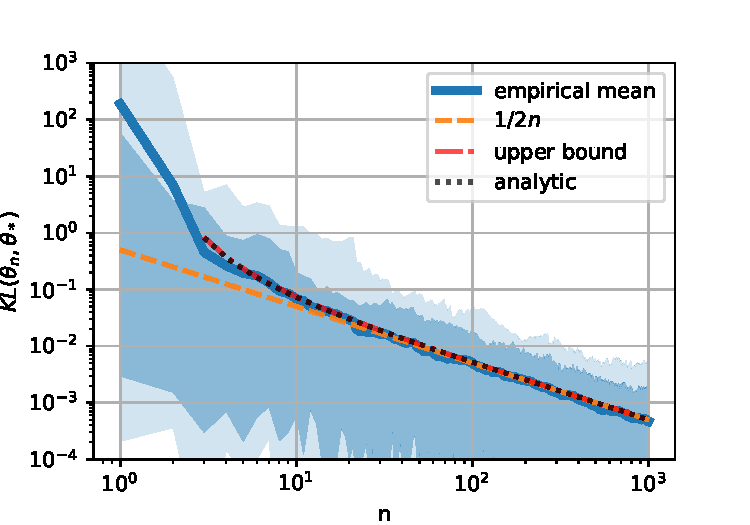
\includegraphics[width=.48\textwidth]{asymptote.pdf}
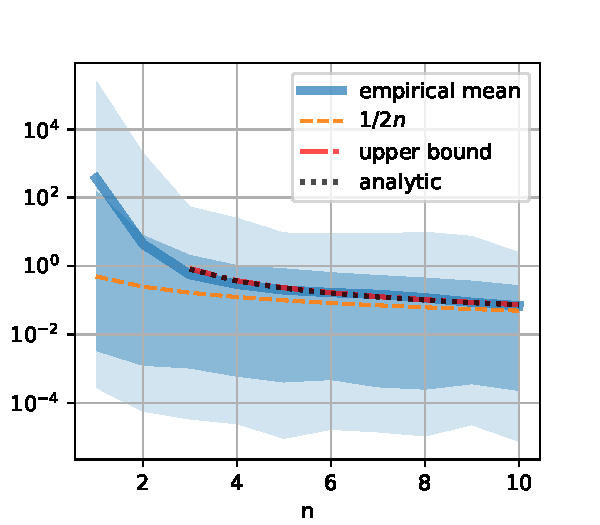
\includegraphics[width=.48\textwidth]{fewsamples.pdf}
	\caption{Suboptimality of a Gaussian variance MLE against number of samples $n$. Bold curve is average over 100 trials,  dark shaded area is 90\% (dark) confidence interval, light shade is min-max interval.  
	\textbf{Left:} as $n$ increases, the suboptimality matches the $1/2N$ asymptote.
	\textbf{Right:} the first few samples significantly deviate from this behavior. In fact, for $n=1$ and $n=2$, the expected value is infinite, but we have a closed form solution and a simple upper-bound for $n>2$.
	}
	\label{fig:curves}
\end{figure}




	\begin{theorem}[MLE Tight Bound]
	The MLE of $\cN(0,\mu_*)$ is $\hat \mu_n^\text{MLE} = \inv{n} \sum_i X_i^2 $.
	Its expected suboptimality is infinite when $n\leq 2$, and otherwise upper-bounded as
	\begin{align}
		 \expect{\bregmanconj( \mu_*; \hat \mu_n^\text{MLE}) }
			\leq \inv{2n} +\frac{2}{n(n-2)} \; .
			\label{eq:MLE_rate}
	\end{align}
\end{theorem}

This upper bound is asymptotically tight.
We illustrate its behavior against empirical data in Figure~\ref{fig:curves}.
 There is also a closed form for the multivariate generalization, thanks to the \href{https://en.wikipedia.org/wiki/Inverse-Wishart_distribution}{inverse Wishart distribution} and the \href{https://en.wikipedia.org/wiki/Wishart_distribution#Log-expectation}{expectation of the log-determinant of a Wishart}. The expected value is infinite whenever $n \leq d+1$ where $d$ is the dimension. We do not perform these calculations for now as we want to focus on the simplest possible examples.
 
As for the MAP, we did not manage to get an asymptotically tight upper bound. Nevertheless, using inequality~\eqref{eq:log_bound}, we did get an interesting upper bound. 
To start, let us recall that the MAP of $\cN(0,\mu_*)$ is $\hat \mu_n = \frac{n_0 \mu_0 + \sum_i X_i^2}{n_0 + n}$.
Its expectation is simply $\mu_n= \frac{n_0 \mu_0 + n \mu^*}{n_0 + n}$.
We now present a lemma on its expected inverse.
\begin{lemma}[Expected MAP Natural Parameter]
	Let's define $a=n_0 \frac {\mu_0 }{ \mu^* }$. For any $n\geq 1$, the expectation of the natural parameter of the MAP of $\cN(0,\mu_*)$ is bounded as
	\begin{equation}
		\frac{\mu^*}{\mu_n}
		\leq \expect{\frac{\mu^*}{\MAPm}} 
		= \expect{\frac{\MAPt}{\natp^*}} 
		\leq \frac{n_0 +n}{a+ (n-2)_+}
		\label{eq:theta_expectation_bound}
	\end{equation}
	where $(x)_+ = \max(0,x)$.
\end{lemma}
Note that the lower bound is a simple consequence of the convexity of the inverse function. 
Using this lemma, along with the log upper bound on the logarithm~\eqref{eq:log_bound}, we get a convergence rate for the MAP. 

\begin{theorem}[MAP Bound]
 Let us  define
 \begin{align}
	b = \frac{(1 + \inv{n_0} - \frac{\mu_0}{\mu^*})^2}{2 (\frac{\mu_0}{\mu^*}+\frac{(n-2)_+}{n_0})(1 + \frac{n}{n_0} )} \; .
 \end{align}
The expected suboptimality of the MAP of $\cN(0,\mu^*)$ with prior hyper-parameters $(n_0,\mu_0)$ is
 \begin{equation}
	\expect{\bregmanconj( \mu_*; \hat \mu_n^\text{MAP})}
	\leq \begin{cases}
		\inv{2(n_0+1)}  +  b\ \text{if}\ n=1,\\
		\frac{1}{n_0 \frac{\mu_0}{\mu^*} +n-2} + b \ \text{if}\ n\geq 2
	\end{cases}
	\label{eq:MAP_rate}
\end{equation}
\end{theorem}

This inequality highlights a clear variance-bias decomposition.
In particular, there is no bias term when $\frac{\mu_0}{\mu^*} =1 + \inv{n_0} $, which happens when the prior is slightly larger than the ground truth.  For instance, when $n_0=1$, it encourages us to set $\mu_0 = 2 \mu^*$.
Remark that the variance term is not asymptotically tight as the log-inequality we used \eqref{eq:log_bound} is not quadratically tight around $1$. We are basically losing a factor 2 compared to $1/2n$.

Using the same bound on the log~\eqref{eq:log_bound}, we  get a loose bound on the MLE, which is useful for comparison purposes.
We relate these loose convergence rates of MAP and MLE in Figure~\ref{fig:MAP_rate}.

\begin{corollary}[MLE Loose Bound] When $n\geq 2$, the MLE expected loss is upper bounded as
\begin{equation}
	\expect{\bregmanconj( \mu_*; \hat \mu_n^\text{MLE}) }
	\leq \inv{n-2} \; .
	\label{eq:MLE_loose_rate}
\end{equation}
\end{corollary}



\begin{figure}[ht]
	\centering
	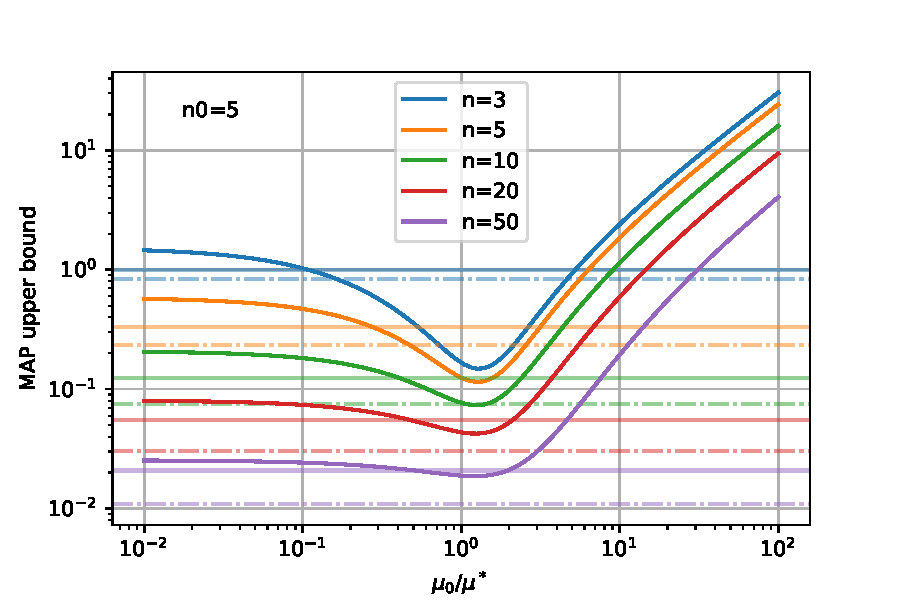
\includegraphics[width=.7\textwidth]{figs/MAP_rates/MAP_rate_n0=5.pdf}
	\caption{
	Convergence rate of MAP~\eqref{eq:MAP_rate} 
	\label{fig:MAP_rate} against the ratio between initialization and optimum $ \frac{\mu_0}{\mu^*}$. 
	We also report the tight convergence rate of MLE~\eqref{eq:MLE_rate} (dash-dotted horizontal lines), and the loose upper bound~\eqref{eq:MLE_loose_rate} (horizontal lines). 
	We report these curves for various values of $n$, and $n_0=5$. 
	We observe that the rate of MAP is significantly better (lower) than the rate of MLE, only when we guessed $\mu_0$ right, within an order of magnitude from $\mu^*$, and for a small number of sample ($n<10$). 
	This observation hints towards the optimality of MLE for large $n$. 
	It makes me feel very interested in convergence rates of MAP in the overparametrized regime $n<\dim(T(X))$.
	}
\end{figure}



\bibliographystyle{apalike}
\bibliography{../references.bib}




\clearpage
\section{Plan}

\begin{enumerate}
	\item intro to exponential family, and density estimation
	\item the thing we want to bound
	\item Examples : gaussian mean and gaussian variance (+other examples, just mentioned)
	\item Insight : Strongly convex case. (+ self-concordance that is not verified either)
	\item insight : bias-variance decomposition
	\item Optimization perspective : SBPP or SBG. But no analysis hold, revealing a flaw of all these techniques.
	\item Discussion : we believe finding a convergence rate would bring new tools useful to deal with common objects such as barrier losses.
\end{enumerate}

Open questions
\begin{itemize}
	\item does a base measure change anything ?
	\item is there multiple conjugate priors ?
	\item misspecified case. Do we have a   formula ?
\end{itemize}


\section{Stuff to cite and why }


\begin{itemize}
	\item Stochastic and online mirror descent: 
	We obviously have rates in this setting, but they all assume 
	that the reference function is strongly-convex relative to a norm. 
	\citep[e.g.][Thm 4.2]{bubeck2015convex}
	\item What is mirror descent called in the literature?
		\begin{itemize}
			\item Mirror Descent \citep{nemirovski1983problem,beck2003mirror} 
			\item NoLips \citep{bauschke2017descent}
		\end{itemize}
	\item Interest in mirror descent boosted by the relatively smooth view 
	of \citet{bauschke2017descent,lu2018relatively}	
	\item 
	The oroblems on how to deal with Bregman divergences abound in optimization, 
	beyond stochasticity. 
	For example, we haven't yet figured out the analog of Nesterov-type acceleration 
	on relatively smooth and strongly convex problems, 
	to bring the convergence rate from linear in $(1-\kappa)$ to $(1-\sqrt{\kappa})$, 
	or just from $1/T$ to $1/T^2$ 
	in the (non-strongly) convex case.
	\citet{dragomir2021optimal} show that naïve application of Bregman updates can not achieve acceleration.
	The tools developped to make progress on one problem might help make progress on the other. 
	\item 
	Stochastic mirror descent in the relatively smooth setting;
	\citet{hanzely2018fastest},
	\citet{dragomir2021fast}
	and the zoo of assumptions
	\item Something about the statistical asymptotic behavior for the MLE? 
	\begin{equation}
		D_A(\theta_*, \theta_n) \approx \frac{1}{2}\norm{\theta_n - \theta_*}_{\nabla^2 A(\theta_*)}^2 
		\approx \frac{1}{n}?
	\end{equation}
	\item Something about how the Bregman divergence is often not considered in the statistics lit 
	because it can be infinite and is non-symmetric and not nice to work with, 
	and so folks focus on $\expect{\norm{\theta_n - \theta_*}^2}$ even if it's somewhat meaningless 
	in the non-asymptotic regime, 
	and the best non-asymptotic results 
	still rely on Taylor expansions after $n > $ something big?
	\item Something about how we don't even know how to deal with decreasing step-sizes 
	of the order of $1/t$ 
	\item 
	Should cite Bach's line of work on SGD, averaging schemes and self-concordant functions https://www.di.ens.fr/~fbach/bach_ejs_self_concordance.pdf
	that obtain the $1/t$ rate in the smooth, convex setting instead of $1/\sqrt{t}$, 
	which is the ``expected'' rate for that setting, 
	and how this approach above is a generalization beyond the Euclidean noise model 
	http://proceedings.mlr.press/v99/marteau-ferey19a/marteau-ferey19a.pdf
	http://proceedings.mlr.press/v99/ostrovskii19a/ostrovskii19a.pdf
\end{itemize}





\end{document}